\documentclass{../template/texnote}

\title{\textbf{What are Galaxies?}}

\begin{document}
    \maketitle \currentdoc{note}
    %<*note>
%\section{Discovery of galaxies}
\section{The Milky Way galaxy}
The Milky Way is the distribution of stars in a disc often visible using the naked eye from suitable places on the Earth.
In a previous article, we had seen that until Hubble's discovery in the 1920s, it was believed that the whole of the observable universe was contained in our Milky Way, an island floating in empty infinite space.
After which it was understood that those fuzzy objects seen in the night sky were worlds distant from ours and were replicas of our own galaxy.
\section{Interstellar dust}
%(mistakenly called nebulae)
Initially these fuzzy objects in the night sky were classified together with what we today call as nebulae.
These nebulae or dark patches like the famous Horsehead Nebula are actually regions of dust concentration.%It is also this dust that leads to the dark patches seen with our galaxy and not the absence of stars.
The dark patches often seen within our galaxy are due to this dust and not the absence of stars as was thought to be the case earlier.
Interstellar dust may contain graphite, silicates and solid hydrogen.
Dust reduces the intensity of star light through absorption and scattering.
	\begin{figure}
	\begin{center}
		\includegraphics[width=\textwidth]{Linn/Dark_Rift_2012.jpg}
	\end{center}
	\caption{Image showing the most prominent dark lane in our galaxy which stretches from the constellations Cygnus to Sagittarius called the Great Rift or the Dark Rift. Image Courtesy: NASA}
	\label{fig:galaxy}
	\end{figure}
	
\section{Rotation and the Presence of Gas}
The diameter of the disc of the Milky Way is estimated to be $\sim$ 30 kpc and its thickness $\sim$ 1 kpc.
The galaxy rotates about it's polar axis, however not like a rigid body.
Figure \ref{fig:rotation} shows a typical rotation curve.
At a distance r from the center O of the galaxy, a circular Keplerian orbit will have a velocity given by,
$$ v = \sqrt{\frac{GM(r)}{r}} $$
	\begin{figure}
	\begin{center}
		\includegraphics[width=\textwidth]{Linn/rotation_curve.png}
	\end{center}
	\caption{Rotation curve of a spiral galaxy. The dotted curve shows how the rotation curve should have sloped down had the entire mass of the galaxy  been confined to its visible boundary. Image Courtesy: J. V. Narlikar, Introduction to Cosmology.}
	\label{fig:rotation}
	\end{figure}
Where M(r) is the mass of the galaxy contained within the radius r and the point A represents the visible extent of the galaxy.
The dotted lines shows how the velocity should have decreased beyond A. However, what we see in practice is the velocity remaining more or less constant upto two or three times the visible boundary.
Some stars like our Sun go around the Galactic Center, whereas some have highly eccentric orbits that takes them out of the galactic plane.
The former type are called population-I stars and the latter are called population-II stars.
The population-II stars are seen to be older than population-I stars.
The mass of our Galaxy is estimated at $\sim 1.4 \times 10 ^{11}$ solar mass.
The absorption lines shown by the spectra of stars in our galaxy show that abosrbing gases are present in the interstellar medium.
The emission nebulae consists of gas that absorbs the UV radiation from stars and radiate it as visible light in spectacular colours.
There are also hot regions near stars which contain hydrogen as H II, ionized by the UV liradiation from stars.
In contrast there are also cool regions containing atomic hydrogen HI.
These were detected using the 21 cm observation in radio astronomy.

%\section{Types of galaxies}
\section{Spirals and Ellipticals}
Galaxies comes in two major types, spirals and ellipticals.
Spirals are probably the most numerous amongst bright galaxies. They show rotation and flattening into a disc like our own galaxy, the presence of a central bulge and dark lanes of absorbing matter.
While spirals are most numerous among bright galaxies, the most numerous of all galaxies are the ellipticals.
They are ellipsoidal in shape, show very little rotation and have very little gas and dust.
Let us revise the modern classification scheme based on the morphology of galaxies that is primarily due to Hubble.
The spirals are arranged in a sequence called Sa, Sb, Sc etc. in decreasing order of the importance of the central nucleus or bulge in relation to the surrounding disc.
Along the sequence, the central spheroid decreases in luminosity and spiral arms become more loosely wound.
Spirals can have bars in the central region and when that happens they are designated SBa, SBb, SBc, etc.
The ellipticals are arranged in a sequence E0, E1, ...E7 based on the progressive flattening of the profiles. E0s have an almost spherical shape and E7s have a lenticular shape.

The distribution of light across galaxies are conveniently described in terms of contours of equal intensity called isophotes.
Another type of galaxy called S0, is intermediate between the ellipticals and spirals.
They have little gas and dust like the ellipticals but their isophotes are similar to those of spirals.
They may have formed from collisions of spirals and ellipticals.
Since the stars are widely spaced they may pass through without problems after the collision but interstellar gas and dust might be thrown out into the intergalactic space.
The isophotes in this case which arise from starlight alone might remain intact.

While this arrangement of galaxies often called the Hubble tuning fork seems to have some order, it is still not known if this represents some evolutionary sequence or not.
In addition to these there exists another class called `irregular' which show no particular pattern.
Until our knowledge in galaxy structure and evolution improves signifcantly these are to be seen as empirical models that can help us better understand the underlying physics. Although we can guess the spiral nature of our galaxy from the presence of the disk, what more can be said about it, given the disadvantage of viewing it from within? What class of spirals does it belong to, and does it have a bar?

%\begin{figure}[ht]
    %\centering
    %\subfigure[The elliptical galaxy ESO 325-G004 part of the Abell S740 cluster.  - Image Courtesy: NASA, ESA, and The Hubble Heritage Team.]{
        %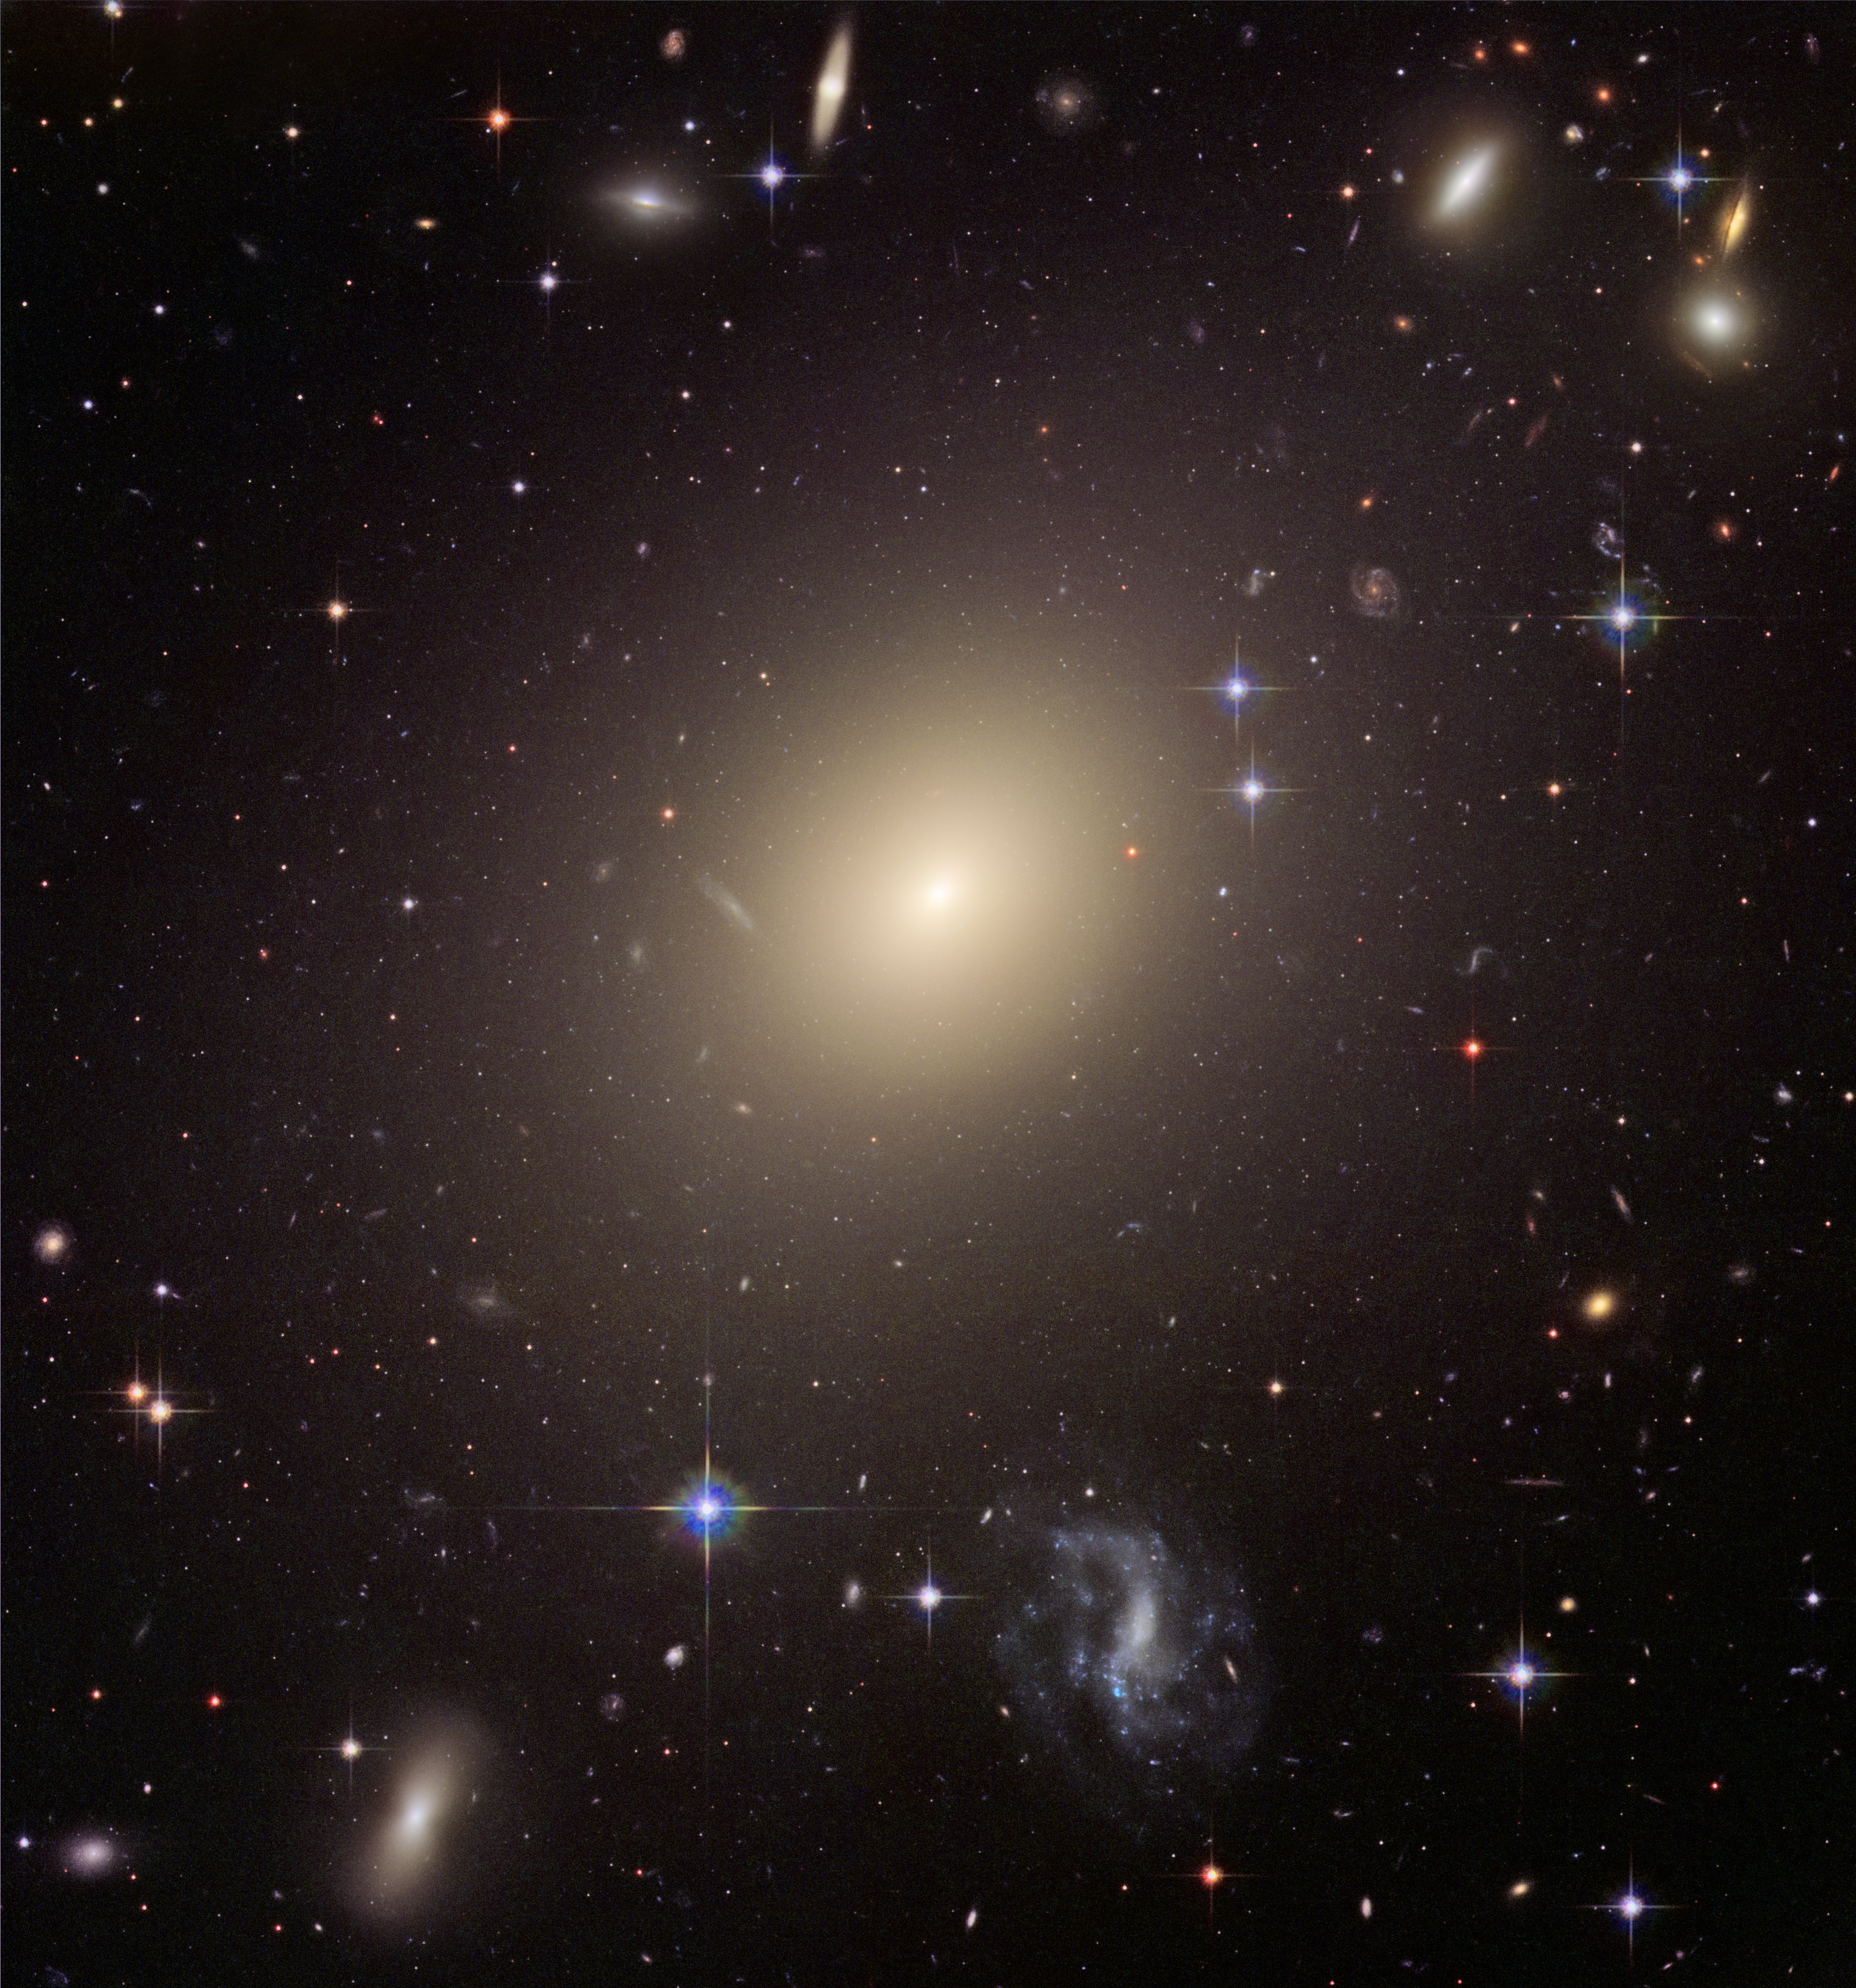
\includegraphics[width=0.63\textwidth]{Linn/Abell_S740,_cropped_to_ESO_325-G004.jpg}
    %}
    %\vspace{1em}
    %\subfigure[Spiral galaxy NGC 1566 - Image Courtesy: Dark Energy Survey]{
        %\includegraphics[width=0.8\textwidth]{Linn/noirlab_noirlab2208a_1024.jpg}
    %}
	%%\caption{}
	%\label{fig:types}
%\end{figure}
\section{Structures on a larger scale}
Galaxies themselves are seen to form patterns on a larger scale. Galaxy groups may contain a few to a few tens of galaxies whereas clusters can contain several hundreds of galaxies.
Galaxies that do not belong to such groups or clusters are called field galaxies.
Our galaxy belongs to a group of $\sim 28$ galaxies, known as the Local Group and are separated by distance of up to $\sim1$ Mpc. Our closest neighbours are the Large and Small Magellanic Clouds at an approximate distance of 50 kpc.
Astronomers have also discovered structures on a much larger scale than clusters. This is done by studying the distribution of clusters across the sky and looking for any grouping or clumping. Larger structures on a scale of $\sim50$ Mpc compared to cluster scales of $\sim5$ Mpc have been discovered. These are called superclusters. Our galaxy belongs to one such supercluster known as the Local Supercluster.
	\begin{figure}
	\begin{center}
		\includegraphics[width=\textwidth]{Linn/From_toddlers_to_babies_RXC_J0032.1+1808.jpg}
	\end{center}
	\caption{Image shows a massive group of galaxies: a cluster named RXC J0032.1+1808. Image Courtesy: ESA/Hubble}
	\label{fig:cluster}
	\end{figure}
	%\nocite{narlikarIntroductionCosmology1993}
	%\nocite{carrollIntroductionModernAstrophysics2014}

    %</note>
    \printbibliography
\end{document}
